% !TEX program = xelatex
% 合并版“四问关系与证据链”图，用于替换 1_restatement.tex 中原来两张重叠的图：
%   ../figures/rigor_pool_20260926/flow_overall_model.pdf
%   ../figures/q1_四问关系与决策边界图.png
% 论文中用法：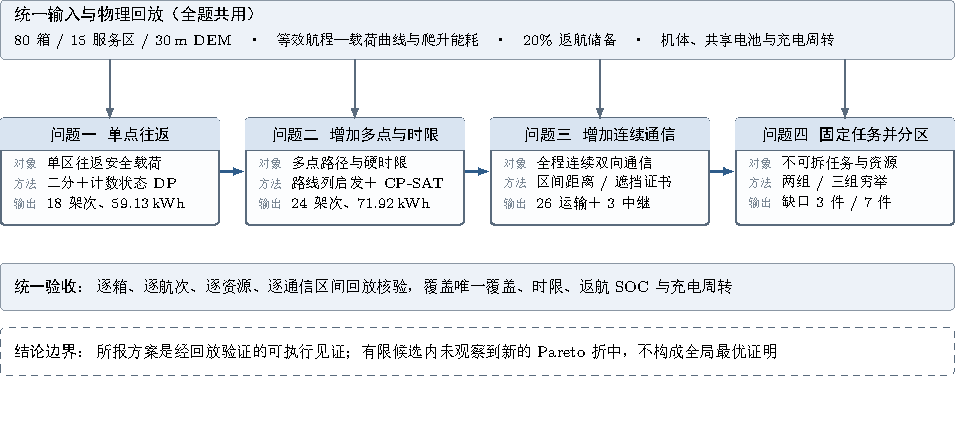
\includegraphics[width=\textwidth]{../figures/fig_roadmap_merged.pdf}
\documentclass[12pt]{ctexart}
\usepackage[margin=0pt,paperwidth=16.5cm,paperheight=7.2cm]{geometry}
\usepackage{tikz}
\usetikzlibrary{arrows.meta}
\pagestyle{empty}

\definecolor{cBand}{HTML}{EDF2F8}
\definecolor{cBox}{HTML}{FCFDFE}
\definecolor{cTitle}{HTML}{D9E4F1}
\definecolor{cLine}{HTML}{5A6B7D}
\definecolor{cAccent}{HTML}{2E5C8A}
\definecolor{cRole}{HTML}{7A8794}

% 每行：6pt 灰色角色标签 + 7pt 内容
\newcommand{\cl}[2]{{\fontsize{6}{7.2}\selectfont\color{cRole}#1}\ \fontsize{7}{9.6}\selectfont #2}
\newcommand{\cln}[4]{\node[anchor=west,align=left] at (#1,#2) {\cl{#3}{#4}};}

\begin{document}
\noindent
\begin{tikzpicture}[x=1cm,y=1cm,every node/.style={inner sep=0pt}]

\def\bw{3.70}    % 阶段框宽度
\def\bh{1.80}    % 阶段框高度
\def\gap{0.45}   % 阶段框间距
\def\xa{0.175}   % 左边距
\def\xb{16.325}  % 右边距
\def\ybox{3.05}  % 阶段框底边
\def\ytop{4.85}  % 阶段框顶边
\def\yone{4.10}  % 内容三行的基线
\def\ytwo{3.76}
\def\ythr{3.42}

%% ================= 顶部：统一输入与物理回放 =================
\filldraw[fill=cBand,draw=cLine!70,line width=0.4pt,rounded corners=2pt]
  (\xa,5.85) rectangle (\xb,6.85);
\node[anchor=west] at (\xa+0.22,6.62)
  {\heiti\fontsize{8}{9.6}\selectfont 统一输入与物理回放（全题共用）};
\node[anchor=west] at (\xa+0.22,6.16)
  {\fontsize{7}{8.4}\selectfont
   80 箱 / 15 服务区 / 30\,m DEM\quad·\quad 等效航程—载荷曲线与爬升能耗\quad·\quad
   20\% 返航储备\quad·\quad 机体、共享电池与充电周转};

%% ================= 四个阶段框 =================
%% 问题一
\pgfmathsetmacro{\bA}{\xa}
\pgfmathsetmacro{\bB}{\xa+1*(\bw+\gap)}
\pgfmathsetmacro{\bC}{\xa+2*(\bw+\gap)}
\pgfmathsetmacro{\bD}{\xa+3*(\bw+\gap)}

\foreach \bx/\ttl in {%
  \bA/{问题一\ \ 单点往返},%
  \bB/{问题二\ \ 增加多点与时限},%
  \bC/{问题三\ \ 增加连续通信},%
  \bD/{问题四\ \ 固定任务并分区}}{%
  \filldraw[fill=cBox,draw=cLine,line width=0.5pt,rounded corners=2pt]
    (\bx,\ybox) rectangle ++(\bw,\bh);
  \begin{scope}
    \clip[rounded corners=2pt] (\bx,\ybox) rectangle ++(\bw,\bh);
    \fill[cTitle] (\bx,\ytop-0.55) rectangle ++(\bw,0.55);
  \end{scope}
  \draw[draw=cLine,line width=0.4pt] (\bx,\ytop-0.55) -- ++(\bw,0);
  \node[anchor=center] at (\bx+\bw/2,\ytop-0.275)
    {\heiti\fontsize{7.5}{9}\selectfont \ttl};
  \draw[-{Latex[length=1.6mm,width=1.2mm]},draw=cLine,line width=0.5pt]
    (\bx+\bw/2,5.85) -- (\bx+\bw/2,\ytop);
}

%% ================= 各阶段内容（对象 — 方法 — 输出） =================
\cln{\bA+0.20}{\yone}{对象}{单区往返安全载荷}
\cln{\bA+0.20}{\ytwo}{方法}{二分 ＋ 计数状态 DP}
\cln{\bA+0.20}{\ythr}{输出}{18 架次、59.13\,kWh}

\cln{\bB+0.20}{\yone}{对象}{多点路径与硬时限}
\cln{\bB+0.20}{\ytwo}{方法}{路线列启发 ＋ CP-SAT}
\cln{\bB+0.20}{\ythr}{输出}{24 架次、71.92\,kWh}

\cln{\bC+0.20}{\yone}{对象}{全程连续双向通信}
\cln{\bC+0.20}{\ytwo}{方法}{区间距离 / 遮挡证书}
\cln{\bC+0.20}{\ythr}{输出}{26 运输 ＋ 3 中继}

\cln{\bD+0.20}{\yone}{对象}{不可拆任务与资源}
\cln{\bD+0.20}{\ytwo}{方法}{两组 / 三组穷举}
\cln{\bD+0.20}{\ythr}{输出}{缺口 3 件 / 7 件}

%% ================= 阶段之间的递进箭头 =================
\pgfmathsetmacro{\ym}{(\ybox+\ytop)/2}
\foreach \i in {0,1,2}{%
  \pgfmathsetmacro{\xs}{\xa+\i*(\bw+\gap)+\bw+0.03}%
  \pgfmathsetmacro{\xe}{\xa+(\i+1)*(\bw+\gap)-0.03}%
  \draw[-{Latex[length=1.7mm,width=1.2mm]},draw=cAccent,line width=0.8pt]
    (\xs,\ym) -- (\xe,\ym);
}

%% ================= 统一验收 =================
\filldraw[fill=cBand,draw=cLine!70,line width=0.4pt,rounded corners=2pt]
  (\xa,1.60) rectangle (\xb,2.40);
\node[anchor=west] at (\xa+0.22,2.00)
  {\fontsize{7.5}{9}\selectfont
   {\heiti 统一验收：}\;逐箱、逐航次、逐资源、逐通信区间回放核验，
   覆盖唯一覆盖、时限、返航 SOC 与充电周转};

%% ================= 结论边界 =================
\filldraw[fill=white,draw=cLine,line width=0.4pt,dashed,rounded corners=2pt]
  (\xa,0.50) rectangle (\xb,1.30);
\node[anchor=west] at (\xa+0.22,0.90)
  {\fontsize{7.5}{9}\selectfont
   {\heiti 结论边界：}\;所报方案是经回放验证的可执行见证；
   有限候选内未观察到新的 Pareto 折中，不构成全局最优证明};

\end{tikzpicture}
\end{document}
